% Created 2022-02-24 qui 14:14
% Intended LaTeX compiler: pdflatex
\documentclass[letterpaper, 11pt]{article}
                      \usepackage{lmodern} % Ensures we have the right font
\usepackage[T1]{fontenc}
\usepackage[utf8]{inputenc}
\usepackage{graphicx}
\usepackage{amsmath, amsthm, amssymb}
\usepackage[table, xcdraw]{xcolor}
\definecolor{bblue}{HTML}{0645AD}
\usepackage[colorlinks]{hyperref}
\hypersetup{colorlinks, linkcolor=blue, urlcolor=bblue}
\usepackage{titling}
\setlength{\droptitle}{-6em}
\setlength{\parindent}{0pt}
\setlength{\parskip}{1em}
\usepackage[stretch=10]{microtype}
\usepackage{hyphenat}
\usepackage{ragged2e}
\usepackage{subfig} % Subfigures (not needed in Org I think)
\usepackage{hyperref} % Links
\usepackage{listings} % Code highlighting
\usepackage[top=1in, bottom=1.25in, left=1.55in, right=1.55in]{geometry}
\renewcommand{\baselinestretch}{1.15}
\usepackage[explicit]{titlesec}
\pretitle{\begin{center}\fontsize{20pt}{20pt}\selectfont}
\posttitle{\par\end{center}}
\preauthor{\begin{center}\vspace{-6bp}\fontsize{14pt}{14pt}\selectfont}
\postauthor{\par\end{center}\vspace{-25bp}}
\predate{\begin{center}\fontsize{12pt}{12pt}\selectfont}
\postdate{\par\end{center}\vspace{0em}}
\titlespacing\section{0pt}{5pt}{5pt} % left margin, space before section header, space after section header
\titlespacing\subsection{0pt}{5pt}{-2pt} % left margin, space before subsection header, space after subsection header
\titlespacing\subsubsection{0pt}{5pt}{-2pt} % left margin, space before subsection header, space after subsection header
\usepackage{enumitem}
\setlist{itemsep=-2pt} % or \setlist{noitemsep} to leave space around whole list
\author{Vinicius Faria}
\date{\today}
\title{Geometria analítica\\\medskip
\large \emph{Anotações Práticas}}
\hypersetup{
 pdfauthor={Vinicius Faria},
 pdftitle={Geometria analítica},
 pdfkeywords={},
 pdfsubject={},
 pdfcreator={Emacs 27.2 (Org mode 9.5.2)}, 
 pdflang={English}}
\begin{document}

\maketitle
\tableofcontents


\section{Espaços vetoriais e subvetoriais}
\label{sec:orgd27b312}
\subsection{Espaços vetoriais}
\label{sec:org07656b4}
Dado um conjunto V, V é um espaço vetorial real caso satisfazer as condições:
\textbf{OBS:} Nas equações abaixo, \(\forall x,y,z \in V\) e \(\forall \alpha , \beta \in \realbb{R}\)
\begin{enumerate}
\item \(x + y = y + x\) (Associatividade)
\item \((x+y)+z = x + (y+z)\) (Comutatividade)
\item \(\exists \theta \in V \ / \ x + \theta = \theta + x = x\) (Existencia do vetor nulo)
\item \(-x \in V \ / \ x + (-x) = \theta\) (Elemento simétrico da soma)
\item \(\alpha (x+y) = \alpha x + \alpha y}\) (Distribuitividade)
\item \((\alpha + \beta)x = \alpha x + \beta x\) (Distruibitividade)
\item \((\alpha \beta) x = \alpha (\beta x)\) (Associatividade)
\item \(1x = x\) (Elemento neutro).
\end{enumerate}

Um espaço vetorial que contém os numeros complexos é denominado \textbf{espaço vetorial complexo}

A partir das expressões acima, é possivel extrair as afirmações:
\begin{enumerate}
\item \(\alpha \theta = \theta\)
\item \(0 \dotc x = \theta\)
\item \(\alpha x = \theta , então \ \alpha = 0 \ ou \ x = \theta\)
\item \((-\alpha )x = \alpha(-x)\)
\end{enumerate}

Alguns exemplos de espaços vetoriais, considerando operações normais:
\begin{itemize}
\item \(V = K_n(x) = {P_r(x) / r \le n}\)
\item \(V = C[a,b]\) \textbf{OBS:} \((f+g)(x) = f(x) + g(x)\) e \((\alpha f)(x) = \aplha f(x)\)
\item \(V = \realbb{R}^n\)
\item \(V = M_{mxn}\)
\end{itemize}

Não são espaços vetoriais:
\begin{itemize}
\item \(V = \realbb{Z}\)
\item \(V =\) Conjunto de polinômios de grau 3
\item Alguns conjuntos com operações diferentes do normal. Ex: \(\alpha x = \alpha (x_1, x_2) = (\alpha ^2 x_1, \alpha x_2)\)
\end{itemize}

\subsection{Subespaços vetoriais}
\label{sec:orgddd055a}
\subsubsection{Definições}
\label{sec:org62f49b5}
Dentro de um espaço vetorial V, há subconjuntos W que são espaços vetoriais menores, contidos em V. \textbf{Todo espaço vetorial possui 2 subsespaços triviais:} Sub. nulo e ele mesmo.
Critérios para subespaços vetoriais:
\begin{enumerate}
\item \(\theta \in W\)
\item \(\forall x, y \in W \rightarrow x + y \in W\)
\item \(\forall \alpha \in \realbb{R}, \forall x \in W \rightarrow \alpha x \in W\)
\end{enumerate}
São subespaços:
\begin{itemize}
\item Soluções lineares homogêneas
\item Qualquer sistema que adote multiplicações/adições usual com a presença do vetor nulo
\end{itemize}
Não são subespaços:
\begin{itemize}
\item Geralmente sistemas com alguma multiplicação/adição fora do comum ou muito específicas (ex. Conjunto de polinomios de terceiro grau)
\item \(u + v = (u_1 , u_1^2) + (v_1, v_1^2)\)
\end{itemize}
\subsubsection{Teoremas}
\label{sec:org257be91}
\textbf{Interseccão de subespaços}. Dado \(W_1 \  e \  W_2\) subespaços vetorias de V, \(W_1 \cap W_2\) também é subconjunto de V. Ex - Matriz triangulares inferiores e superiores.

\textbf{Soma de subespaços}. Dado \(W_1 \  e \  W_2\) subespaços vetoriais de V, \(W_1 + W_2\) também é subconjunto de V. Caso \(W_1 \cap W_2 = \theta\), a soma é chamada de \textbf{soma direta}, denotada por \(W_1 \oplus W_2\)


\section{Combinação linear}
\label{sec:orgff4212c}
Dado um espaço vetorial V, o vetor \(v \in V\) é considerado a combinação linear de \(v_1 + v_2 + ... v_n\) caso houver escalares \(\alpha_1 ... \alpha_n\) tais que:

\begin{center} $v = \alpha_1v_1 + ... + \alpha_nv_n$ \end{center}

*Toda combinação de 3 vetores com sistema em SPI que não são multiplos entre si formam \(\realbb{R}^3\)

Em exercícios envolvendo combinação linear, dado v e \(v_1 ... v_n\), colocar tudo em um sistema e resolver (escalonando ou manualmente). \textbf{Caso o sistema for possível e determinado, é uma combinação linear,
caso contrário (por desigualdades depois de substituir valores, por exemplo) não é uma combinação linear}.

Como exemplo, utilizando os vetores \(v_1 = (1,-1,3) \ e \ v_2 = (2,3,0)\) para a combinação linear, verificar se podem ser combinados para formar: \(u = (3,3,3) \ e \ v=(-2,-8,6)\).

\begin{itemize}
\item \(u\) não pode ser formado, pois, dependo da maneira que o sistema for resolvido \(\alpha_2 = 1\) ao mesmo tempo que \(\alpha_2 = \frac{4}{3}\), classificando o sistema como impossível.

\item Agora, \(v\) é totalmente possível, pois ao escalonar ou tentar resolver o sistema claramente chegamos em \(\alpha_1 = 2\) e \(\alpha_2 = -2\).
\end{itemize}

\subsection{Subespaço gerado}
\label{sec:orge7d8bc9}

Dado um conjunto de vetores S (combinação linear), o subespaço vetorial formado por S é chamado de \textbf{subespaço gerado} por S. Assim os vetores \(s_1, s_2 ... s_n\) \textbf{geram} ou formam um \textbf{conjunto gerador}
de um espaço vetorial V se V coincide com o subespaço. Ou seja \(S \subset V\) e \(V \subset S\).

De modo prático devemos mostrar que cada vetor composto por S pertence a V, e que qualquer vetor de V pode ser composto por combinação linear dos vetores que compõem S.

Para a resolução de exercícios, primeiro provar a primeira hipótese, depois verificar se o sistema formado possui uma única solução (se houver infinitas ou nenhuma solução, não é um subespaço gerado).

\textbf{EX:} \(\alpha_1(1,0,0), \alpha_2(0,1,0) \ e \ \alpha_3(0,0,1)\) formam um subespaço, pois o sistema montado é SPD.

\textbf{EX2:} \(\alpha_1(1,3,-2), \alpha_2(-1,2,1), \alpha_3(5,0,-7)\) não formam um subespaço, pois o sistema abaixo não possui solução

\begin{center}
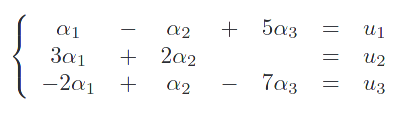
\includegraphics[width=.9\linewidth]{./img/sist1.png}
\end{center}

\subsection{Dependência linear}
\label{sec:orgee4002c}
O conceito de dependência linear determina qual o menor conjunto gerador de um espaço vetorial. Dado V um espaço vetorial e os vetores \(v_1 ... v_n\), se há numeros reais \(\alpha_1 ... \alpha_n\) tais que \(\alpha_1 v_1 + ... + \alpha_n v_n = \theta\), ou seja, há numeros reais multiplicados pelos vetores, que quando somados, dão o vetor nulo, dizemos que são \textbf{Linearmente dependentes}
Note que sempre há a solução trivial para essa conta dada, portanto se a unica solução para o sistema for a trivial (todos \(\alpha = 0\)), o sistema é considerado \textbf{linearmente independente}.

Algumas observações para facilitar exercícios:
\begin{itemize}
\item Dado \(\realbb{R}^n\) e n vetores que não são multiplos entre si, eles formam o espaço \(\realbb{R}^n\).
\item Dado \(\realbb{R}^n\) e r vetores, se \(r > n\), então os vetores r serão LD. Note que se  \(r < n\) não vale a mesma afirmativa, pois ao escalonar o sistema há a possibilidade de anular linhas, já que o sistema é homogêneo. (Ex 4.25 do livro)
\item Colocando as váriaveis no sistema A, se \textbf{det(A) = 0 = SPI = LD, ou det(A) \(\ne\) 0 = SPD = LI}
\item \textbf{Se o sistema contêm o vetor nulo, ele é linearmente dependente.}
\end{itemize}

\textbf{Teorema:} Dado um conjunto LD \{\(v_1...v_n\)\}, algum elemento \(v_i\), não nulo, é uma combinação linear dos outros.

\begin{center}$0 = \alpha_1v_1 + ... + \alpha_iv_i + ... + \alpha_nv_n \\$ 
$-\alpha_jv_j = \alpha_1v_1 + ... + \alpha_nv_n$ \end{center}

Assim, dado \(V = \realbb{R}^3\), \(v_1,v_2,v_3 \in V\), \{\(v_1,v_2\)\} é LD somente se pertencerem á mesma reta de origem, com \(v_n \in\) \{\(\beta_xv_x; \beta \in \realbb{R}\)\}. \{\(v_1,v_2,v_3\)\} é LD somente se pertencerem ao mesmo plano que passa pela origem, \(v_n \in\) \{\(\beta_1v_x + \beta_2v_y;\beta_i \in \realbb{R}\)\}.


\section{Bases}
\label{sec:org746b596}
Determinar um conjunto de vetores que gere um espaço vetorial V de tal modo que todos os vetores sejam necessários para gerar V.

Dado um espaço vet. V e B = \{\(u_1,u_2, ... ,u_n\)\}, dizemos que B é uma base de V se:
\begin{itemize}
\item Os vetores de V são \textbf{LI}
\item B for gerador de V
\end{itemize}

Em outras palavras, verificar primeiro se o conjunto é LI, escalonando a matriz homogênea e verificando que a solução trivial é a unica (ou pelo método de determinantes. Depois, escalonar 
sistema para obter valores quaisquer de V \((v_1, v_2, ... , v_n)\), e verificar que ele é SPD. Se as duas condições forem aceitas, B é uma base para V.

\textbf{Uma base de \(\mathbb{R}^n\) deve conter, obrigatoriamente, exatamente \(n\) vetores.} Dado um numero de p vetores, se p > n, o sistema vai ser LD, se p < n, o sistema pode até ser LI, mas não irá gerar V (sistema impossível).

\subsection{Dimensão de um espaço vetorial}
\label{sec:orgf000553}
Um espao vetorial V tem dimensão n em símbolo, dim n, quando:

\begin{itemize}
\item Existem n vetores linearmente independentes.
\item (n+1) vetores são sempre linearmente independentes.
\end{itemize}

Ou seja, a dimensão de um espaço vetorial V é definida como sendo o número de vetores de uma base de V. Assim, podemos extrair algumas informações:
\begin{itemize}
\item Uma base \(\mathbb{R}^n\) tem dimensão n
\item Uma base \(M_{nxn}\) possui \(n^2\) elementos e dimensão.
\item Uma base \(K_n(x)\) possui n+1 elementos e dimensão.
\end{itemize}

\textbf{Teorema:} Se x e y são duas bases de um espaço vetorial V. Se x é uma base de com n vetores V, ela gera V, assim y também possui exatamente n vetores, pois caso contrário, os vetores serão LD. Qualquer base de um espaço vetorial V possui o mesmo número de elementos

\textbf{Teorema 2:} Qualquer conjunto de vetores LI de um espaço vetorial V de dimensão finita está contido em uma base de V. Ou seja se dim \(V = n\), qualquer conjunto LI com n vetores formará uma base de V

\subsubsection{Dimensão de subespaços}
\label{sec:org4afc3d6}
Determinar a dimensão de um subespaço vetorial e completar a base de um subespaço para obter uma base de um espaço vetorial. Tendo base que as linhas não nulas em uma matriz escalonada
são sempre \textbf{LI}. Se W é subespaço vetorial V de dimensão n, \(dim \ W \le n\), e se \(dim \ W = n\), então \(W = V\). W não pode conter mais de n vetores, se não será LD.

\begin{itemize}
\item Se dim W = 0, então W é um ponto
\item dim W = 1, reta passando pela origem
\item dim W = 2, então W é um plano passando pela origem
\item dim W = 3, então W é igual ao \(\mathbb{R}^3\)
\end{itemize}

\textbf{Teorema:} \(dim(W_1+W_2) = dim W_1 + dim W_2 - dim(W_1\cap W_2)\). Dado 2 planos, por exemplo \(\pi_1: x+y-z=0\) e \(\pi_2: x=y\), obtemos \(\pi_1 = [(1,0,1),(0,1,1)]\) e \(\pi_2 = [(1,1,0),(0,0,1)]\), cuja interseção é uma reta. Assim, a adição dos 2 gera \(\mathbb{R}^3\).

\textbf{Teorema 2}: Dado uma base e seus vetores, existe uma única n-upla de escalares que resultam em v.

Para determinar as bases e a dimensão de W, colocamos os vetores de W em uma matriz, porém \textbf{um vetor por linha (em vez de coluna!)}, ao contrário que foi feito até agora. Se uma das
linhas forem nulas, a base de W será a vetores de forma escalonada. Caso contrário, será os vetores originais. Na hora de \textbf{completar bases}, é necessário observar, dado \(V = \mathbb{R}^n\),
se W possui n linhas (vetores) não nulos na \textbf{forma escalonada}, caso contrário, é so "preencher" com vetores canônicos até completar n vetores.

\textbf{Ex com linhas nulas:}

\(V = \mathbb{R}^4\), \(W = \{(1,0,1,2),(2,1,1,0),(0,-1,1,4)\}\) um subespaço de V. Escalonando a matriz temos

\begin{center} $\begin{pmatrix} 1 & 0 & 1 & 2 \\ 0 & 1 & -1 & -4 \\ 0 & 0 & 0 & 0 \end{pmatrix}$ \end{center}

Assim, W tem dimensão 2 e \((1,0,1,2), (0,-1,-1,-4)\) são a base para W, e caso necessário completar a base, adicionamos os vetores \((0,0,1,0),(0,0,0,1)\), tornando esses vetores uma base para \(\mathbb{R}^4\)

\textbf{Ex sem linhas nulas:}

Base para o \(\mathbb{R}^2\), que contenha os vetores: \(u = (1,2,3)\), \(v=(2,1,1)#\), escalonando a matriz:

\begin{center} $\begin{pmatrix} 1 & 2 & 3 \\ 0 & 3 & -5 \end{pmatrix}$ \end{center}

Então, já que não há linhas nulas, podemos simplesmente declarar como vetores de W \((1,2,3),(2,1,1)\).

\textbf{OBS:} em casos de matrizes \(\begin{pmatrix} 1 & -5 \\ -4 & 2 \end{pmatrix}\), colocamos na matriz para escalonar na forma \(\begin{pmatrix} 1 & -5 & -4 & 2 \end{pmatrix}\).

\subsection{Mudança de base}
\label{sec:org165d1da}
Dado um espaço V e \(v = \alpha_1v_1 + ... + \alpha_nv_n\), chamamos os escalares de \textbf{coordenadas} ou \textbf{componentes} de \(v\) em relação àquela base. Trocando as ordem da base, trocamos a ordem das coordenadas.
Por isso, chamaremos as bases de \textbf{ordenadas} agora em diante.

Visto que as coordenadas de um vetor em uma base dependem da base fornecida, não basta fazer uma combinação linear para converter bases. Assim primeiro calcula-se a \textbf{matriz de mudança de base}, depois encontra-se as novas coordenadas utilzando-a:

Podemos converter uma base \(B = \{u_1,...,u_n\}\) para outra \(B' =\{w_1,...,w_n\}\), para montar a matriz, obter cada \(w\) em razão da combinação linear de \(u\) e colocar na matriz na forma:

\begin{center} $w_1 = a_{11}u_1 + a_{21}u_2 + ... + a_{n1}u_n \\ w_2 = a_{12}u_1 + a_{22}u_2 + ... + a_{n2}u_n \\ ... \\ w_n = a_{1n}u_1 + a_{2n}u_2 + ... + a_{nn}u_n$ \end{center}

Assim, obtemos a matriz \([A]\frac{B'}{B}\) (sem a barra), que é chamada de matriz de mudança de base \(B\) para \(B'\). Multiplicando ela por uma matriz \(M_{1xn}\), preenchidas com \(y_1...y_n\), obtemos os escalares
\(y_n\), que \(x_n = a_{n1}y_1 + ... + a_{nn}y_{n}\). v' é a \textbf{matriz de coordenadas em relação à nova base}.y
Ou seja,
\begin{center} $v = A \cdot v' \\ v' = A^{-1} \cdot v$ \end{center}

Em um sistema de polinômios, por exemplo, os v' são os escalares que multiplicam cada vetor da nova base, cuja ordem varia dependendo de foram distruibuidos eles na hora de montar a matriz.

Fica um exemplo do livro:

\begin{center}
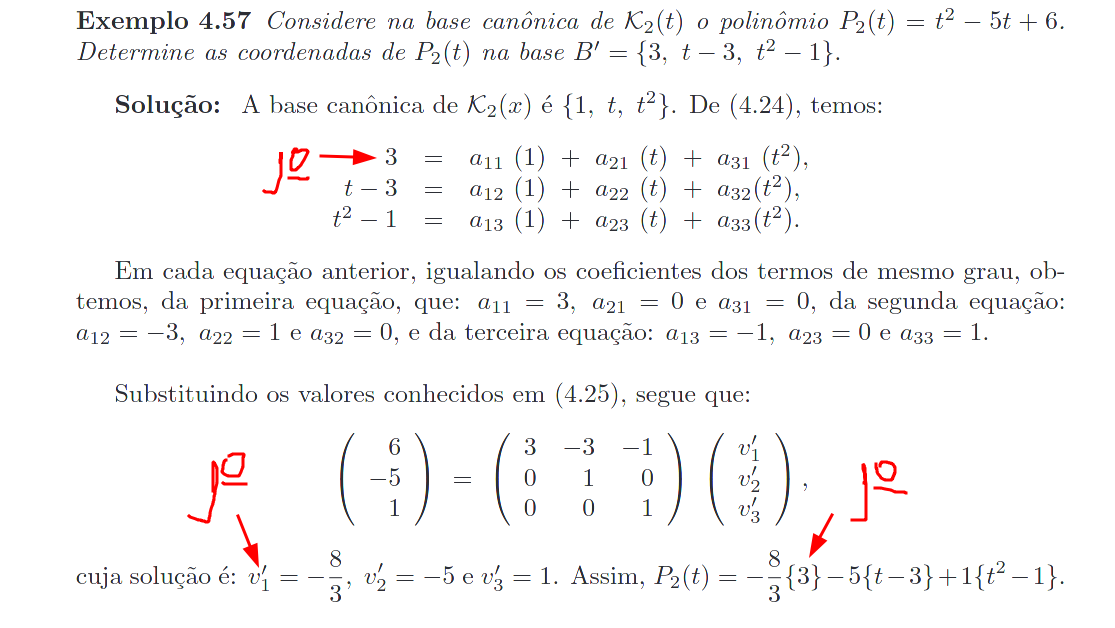
\includegraphics[width=.9\linewidth]{./img/polibase.png}
\end{center}





\section{Transformação linear}
\label{sec:org4e4b6db}
Funções da forma \(v=F(u)\), chamada de transformações lineares. Dado os espaços vetoriais \(U\) e \(V\) e \(F\) uma função que associa um vetor de \(U\) a um único vetor de \(V\), escreve-se \(F : U \to V\).
\textbf{Dizemos que F leva U em V, sendo F uma transformação linear}

Dado um vetor \(u=(u_1,u_2)\), então \(F(u) = (u_1, u_1 + u_2, u_2)\) é uma função que leva o \(\mathbb{R}^2\) em \(\mathbb{R}^3\).

Dado uma \(T: U \to V\), T é uma transformação linear caso
\begin{itemize}
\item \(T(u+v) = T(u) + T(v), \every u, v \in U\)
\item \(T(\alpha u) = \alpha T(u), \every \alpha \in \mathbb{R}\)
\end{itemize}

Assim, podemos afirmar:
\begin{itemize}
\item T é transformação linear se preservado as equações básicas de um espaço vetorial.
\item Se \(U=V\), \(T: V \to V\), \(T\) é um \textbf{operador linear}.
\end{itemize}

Como exemplos:
\begin{itemize}
\item \(T(u) = (u_1,u_2) = (u_1,0)\) é transform.
\item \(T : K_n(x) \to K_{n-1}(x), T(P_r(x)) = \frac{d}{dx} P_r(x)\) é transform.
\item \(T: R^n \to R^m, A_{mxn}, T(u) = Au\) é transform, e a matriz \(A_{mxn}\) sempre determina esse tipo de transformação
\item \(T:U \to V, U=V=C[a,b],T(x) = f(t)x(t)\), sendo \(f(t)\) contínua e fixa e \(x \in V\) é transform.
\item \(T(u) = (u_1-u_2 + u_3, u_2+1)\) não é (primeira propriedade).
\end{itemize}

\subsection{Propriedades da transformação linear}
\label{sec:org11ae21e}
\begin{itemize}
\item \(T(\theta) = \theta\),pois, \(T(\theta) = T(0u) = 0T(u)\) assim, leva o vetor nulo ao vetor nulo.
\item \(T(\alpha u + \beta v) = \alpha T(u) + \beta T(v)\)
\end{itemize}

Uma transformação linear deve atender essas duas propriedades. Muita atenção que obedecer essa primeira propriedade não indica que é obrigatoriamente uma transformação linear.

\textbf{Teorema:} Dado uma base \(\{u_1, ... , u_n\}\) de U, e as imagens \(T(u_1)...T(u_n)\) conhecidas, é sempre possivel obter a imagem de \(T(u)\), pois podemos escrever como uma "combinação" linear.

\begin{center} $u = \alpha_1u_1 + ... + \alpha_nu_n$, multiplicando T pelos dois lados, temos: $\\ T(u) = \alpha_1T(u_1) + ... + \alpha_nT(u_n)$. \end{center}

Passo a passo na pag 223 do livro.

\subsection{Operações com transformações lineares}
\label{sec:orgf6da85e}
No caso da \textbf{adição}, dado que \(T_1\) e \(T_2\) transformadores lineares de \(U\) em \(V\), ou seja, os dois levam de U para V (obrigatoriamente!), temos:

\begin{center} $(T_1 + T_2)(u) = T_1(u) + T_2(u)$ \end{center}

Ou seja, simplesmente somamos as duas funções. Como exemplo: \(T_1 = (u_1 + u_2, u_2), T_2 = (u_2, u_1)\), a soma será \((T_1 + T_2)(u) = (u_1 + 2u_2, u_1 + u_2)\).

Na \textbf{multiplicação}, \((\alpha T)(u) = \alpha T(u)\), ou seja, apenas multiplica-se a função. \(2T(u_1+u_2,u_1) = (2T)(u) = (2u_1 + 2u_2, 2u_1)\).

\begin{itemize}
\item \(T(-u) = -T(u)\)
\item \(T(u-v) = T(u)  - T(v)\)
\end{itemize}

Ja na \textbf{composta}, dado que as duas funções são compatíveis, ou seja, \(T_1 : U \to V, T_2: V \to W\) (T2 toma a "saída" de T1 como "entrada"). A aplicação \(T_2 \circ T_1 = T_2(T_1(u))\) é a operação composta. Dado que as duas
transformações são lineares, a composta também vai ser.

Dado \(T_1, T_2\) transformações lineares de \(U\) em \(V\) e \(S_1,S_2\) de \(V\) em \(W\), então:

\begin{itemize}
\item \(S_1 \circ (T_1 + T_2) = S_1 \circ T_1 + S_1 \circ T_2\)
\item \((S_1 + S_2) \circ T_1 = S_1 \circ T_1 + S_2 \circ T_1\)
\item \(\alpha (S_1 \circ T_2) = (\alpha S_1) \circ T_2 = S_1 \circ (\alpha T_2)\)
\item \(T_1 \circ T_2 \ne T_2 \circ T_1\)
\item \(T_1 \circ T_1\) representado por \(T^2_1\).
\end{itemize}

Ex: Dado \(T_1(u) = (u_1 - u_2, u_2), T_2(u) = (u_1,2u_2)\), Temos \((T_1 \circ T_2)u = T_1(u_1,2u_2) = (u_1 - 2u_2, 2u_2)\).

\textbf{OBS:} Caso as transformações no caso da adição ou composição não forem "compatíveis" como descritas, não são possíveis de ser realizadas.

\subsection{Existência e unicidade de transformações lineares}
\label{sec:org80db819}
Agora, vamos descobrir um certo \(T(u)\), dado \(T: \mathbb{R}^n \to \mathbb{R}^m\), e uma base para \(\mathbb{R}^n\). Assim, \(T(u_1) = v_1, T(u_2) = v_2\), e assim em diante.

Por exemplo, dado \(T: \mathbb{R}^2 \to \mathbb{R}^2\), que satisfaz \(T(1,1) = (2,1,2); T(0,1) = (1,1,2)\). Para descobrir \(T(u)\), dado que \(\{(1,1),(0,1)\}\) é base do \(\mathbb{R}^2\), escrevemos:

\begin{center} $(u_1,u_2) = \alpha(1,1) + \beta(0,1) = (\alpha, \alpha + \beta) \\ \alpha = u_1, \ \beta = u_2 \\ T(u_1,u_2) = T(u_1(1,1) + (u_2-u_1)(0,1)) \\ = u_1(2,1,2) + (u_2-u_1)(1,1,2) \\ = (u_1 + u_2, u_2, 2u_2)$ \end{center}

Lembrando que, para achar um vetor \(T(u) = (x,y)\), basta igualar cada vetor de \(T(u)\) com o vetor igualado, formando um sistema.

Em polinômios, agrupa-se os termos comuns (pg 234.)

\subsection{Imagem da transformação linear}
\label{sec:org287b87b}
Dado \(T: U \to V\), a \textbf{imagem de T}, denotada por \(Im(T)\), é o conjunto de vetores \(v\) em que há um vetor \(u\) em que \(T(u) = v\). A imagem pode ser um plano, uma reta, ou uma expressão.

Por exemplo, dado \(T(u_1, u_2, u_3 = (u_1,u_2,0)\), \(Im(T) = \{(v_1,v_2,0), \forall v_1,v_2 \in \mathbb{R}\}\), ou seja, o plano xy.

Outro exemplo: \(T(u_1,u_2) = (u_1,u_2,\frac{u_1+u_2}{2})\), \(Im(T) = \{(v_1,v_2,v_3) \in \mathbb{R} / v_1 + v_2 -2v_3 = 0\}\).

Em termos gerais, igualamos a expressão de cada vetor de \(T(u)\) para \(v_i\), formando um sistema. Caso o sistema só admita solução para determinados valores, ele só tera imagens para esses valores. Caso contrário \(Im(T) = \realbb{R}^n\). Especificar \textbf{todas} as condições, como no ex 5.12.

\textbf{Teoremas: Transformações e subespaços} (Dado \(T: U \to V\):
\begin{itemize}
\item \(Im(T)\) é subespaço de V
\item \(T^{-1}(S)\) é subespaço de U
\item O conjunto \(\{T(u_1),T(u_2),T(u_3),T(u_n)\}\) gera \(Im(T)\)
\end{itemize}

Um exemplo bem completo para tudo visto é o 5.28 da pág 238.

\subsection{Núcleo da transformação linear}
\label{sec:org7f708a2}
Um núcleo de \(T\), denotado por \(Ker(T)\) ou \(N(T)\), é o conjunto de vetores \(u\) que são levados para o vetor nulo de \(v\). \(N(T) = \{u \in U / T(u) = \theta \in V\}\). Pode ser uma reta, um plano, expressão, etc.
\(Ker(T)\) também é um subespaço de \(V\), dado \(T: U \to V\).

Para encontrar o núcleo, basta igualar a expressão de todos os elementos a 0, formando um sistema. A solução do sistema é o núcleo, lembrando que deve-se especificar \textbf{todas} as condições, inclusive a que dependem de outras. Um exemplo bom é o 5.12, novamente.

\subsection{Dimensão da imagem e do núcleo}
\label{sec:org520f6c4}
Dado uma transformação \(T: V \to W\), a \(dimN(T)\) e \(dimIm(T)\) é correspondente ao número de vetores que compõem cada um dos elementos. Caso \(Im(T) = W\), a dimensão será a mesma de \(W\)

Pegando os 2 exemplos do material:

\begin{center}
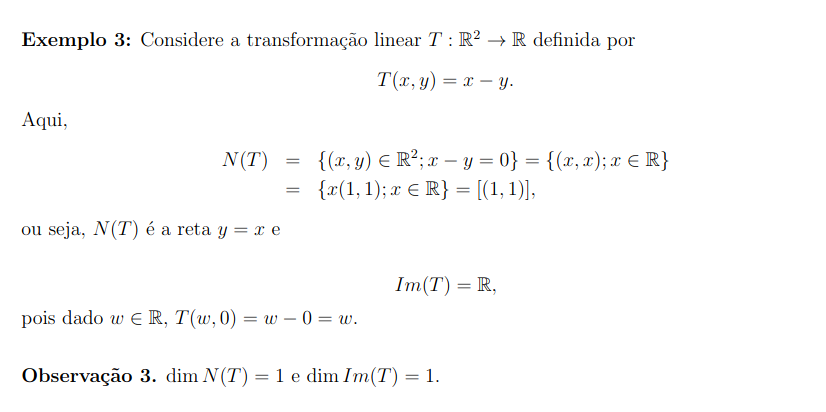
\includegraphics[width=.9\linewidth]{./img/ex3.png}
\end{center}

\begin{center}
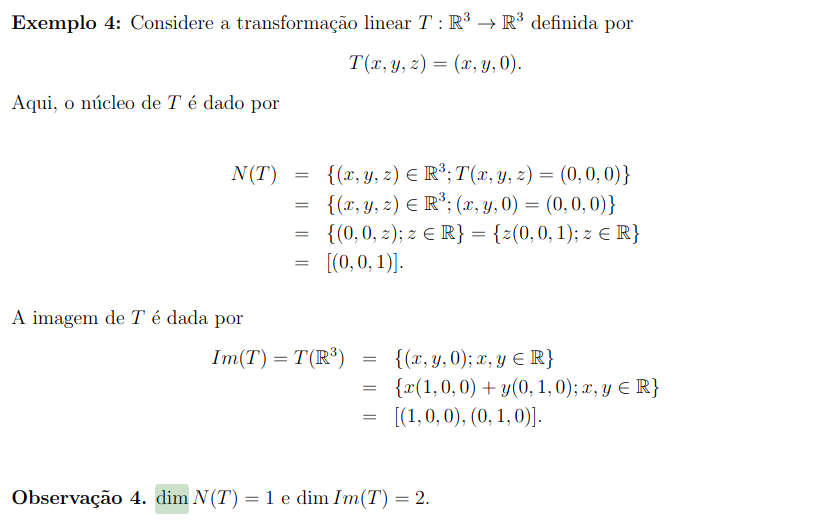
\includegraphics[width=.9\linewidth]{./img/ex4.png}
\end{center}

\textbf{Teorema:} \(dimN(T) + dimIm (T) = dim V\).
\subsection{Isomorfismo}
\label{sec:org5f779a2}
Primeiramente, inciamos o teorema: Uma transformação linear T é injetora se e somente se ela for sobrejetora.

Uma transformação linear \(T: V \to W\) que é injetora e sobrejetora é chamada de isomorfismo, e os espaços são chamados de isomorfos - \textbf{possuem a mesma dimensão}. Todo isomorfismo possui
uma inversa \(T^{-1}\), em que \(T \circ T^{-1} = I\).

Para afirmar que T é injetora. e portanto, sobrejetora, verificar que \(N(T) = \{(0,0,0)\}\). Assim, ela será um isomorfismo.
\subsection{Matriz de uma transformação linear}
\label{sec:org4024d7b}
\end{document}